% Unterstützung für Links und PDF Metadaten
\input{header.tex}
% Einstellungen hier, z.B. Fonts



\begin{document}
% Text hier
\title{V27 – Zeeman-Effekt}
\date{Durchführung: 08.01.2020, Abgabe: 19.01.2020}

% 7 \, s vor Korrekturabgabe:

\maketitle
\tableofcontents
\newpage

\section{Zielsetzung und Theorie}

\subsection{Zielsetzung}
Da Messungen von quantenmechanischen Systemen sich aufgrund ihrer geringen Größe und aufgrund der heisenbergschen
Unschärferelation als höchst schwierig erweisen,
sollen in diesem Experiment analoge, makroskopische Systeme untersucht werden. Dazu werden akustische Modelle genutzt,
die die Wellenfunktionen von Elektronen in einem Wasserstoffatom, Wasserstoffmolekül oder in einem 1-D Festkörper
simulieren können.


\subsection{Theorie}
\subsection{Die Americium-Quelle}

Am241 ist ein $\alpha$-Strahler. Das heißt, es werden Helium-Kerne bestehend aus zwei Protonen und zwei Neutronen emittiert,
die in diesem Versuch anschließend auf eine Goldfolie treffen. Das Zerfallsschema ist in Abbildung \ref{fig:zerfall} zu sehen.
Das Americiumatom zerfällt also in ein $\alpha$-Teilchen und in ein Np237-Atom.

\begin{center}
  $^{95}_{241}$Am \rightarrow $^{93}_{237}$Np + $^{2}_{4}$He
\end{center}

Aufgrund des Massendefekts wird beim Zerfall Energie frei, die sich als kinetische Energie der beiden Zerfallsprodukte
manifestiert. Das Americium kann direkt in den Grundzustand des Np237 zerfallen (was jedoch sehr unwahrscheinlich ist, siehe Abbildung
\ref{fig:zerfall}) oder zunächst in einen angeregten Zustand. Durch das Emittieren von Photonen kann dann der Grundzustand
erreicht werden.

\begin{figure}
\centering
\includegraphics[width=0.7\textwidth]{zerfall.png}
\caption{Zerfallsschema von Am241 \cite{gsi}.}
\label{fig:zerfall}
\end{figure}

\subsection{Wechselwirkung in Materie}

Geladene Teilchen wie die $\alpha$-Teilchen wechselwirken in einem Medium mit den Atomen in diesem Medium. Da $\alpha$-Teilchen
eine große Masse und elektrische Ladung besitzen, wechselwirken sie stark mit den Atomen in ihrer Umgebung, sodass ihre
Reichweite stark begrenzt ist. Des Weiteren hängt ihre Reichweite von der Dichte des Materials ab.
Ein dickeres Blatt Papier oder ein Abstand von wenigen Zentimetern zur Strahlungsquelle reicht somit schon aus, um sich vor der
$\alpha$-Strahlung zu schützen.

Eine Wechselwirkung kann zum Beispiel durch Anregung der Atome im Material stattfinden. Eine andere Möglichkeit liegt darin,
dass ein $\alpha$-Teilchen ein Atom ionisiert. Die Strahlung verliert dabei an Energie und die Teilchen erfahren eine
Richtungsänderung.

\begin{figure}
\centering
\includegraphics[width=0.7\textwidth]{rutherfordschema.png}
\caption{Schema zum Rutherfordversuch \cite{unigoett}.}
\label{fig:streu}
\end{figure}

Der Energieverlust pro Weglänge kann durch die Bethe-Bloch-Formel berechnet werden. Sie gilt jedoch nur für niedrige
Energien.

\begin{equation}
\frac{\mathrm{d}E}{\mathrm{d}x}=\frac{4\pi e^4z^2n Z}{m_ev^2(4\pi\epsilon_0)^2}\log{\left(\frac{2m_ev^2}{I}\right)}
\end{equation}

Dabei ist $Z$ die Ladungszahl des Mediums, $n$ die Anzahl der Atome pro $m^3$, $I=Z*10$eV die mittlere Ionisationsenergie,
$z$ die Ladungszahl der $\alpha$-Teilchen und $m_{\alpha}$ die Masse der $\alpha$-Teilchen. $v$ ist ihre Geschwindigkeit.

Somit beträgt beispielsweise das Bremsvermögen der Teilchen in Luft (genähert als reines Stickstoff)

\begin{equation}
\frac{dE}{dx}=\SI{0,4}{\mega\electronvolt} .
\end{equation}

Die Bethe-Bloch-Formel kann außerdem so umgeformt werden, dass die Reichweite d$x$ bestimmt werden kann:

\begin{equation}
dx = dE\frac{4\pi m_e v^2\epsilon^2_0}{e^4z^2nZ}\log^{-1}\left(\frac{2m_e v^2}{I}\right) .
\end{equation}

\subsection{Der Wirkungsquerschnitt}

Der Wirkungsquerschnitt ist ein Maß für die Wahrscheinlichkeit, dass zwei Teilchen miteinander wechselwirken. Der differentielle
Wirkungsquerschnitt beschreibt dabei die Intensitätsverteilung über alle Raumrichtungen $\Omega$.

Mit Hilfe der Rutherfordschen Streuformel kann die Wahrscheinlichkeit berechnet werden, dass ein gestreutes Teilchen nach der
Ablenkung um einen Winkel $\theta$ im Raumwinkel d$\Omega$ auftritt.

\begin{equation}
\frac{\mathrm{d}\sigma}{\mathrm{d}\Omega}(\theta)=\frac{1}{(4\pi\epsilon)^2}\left(\frac{z Z e^2}{4 E_{\alpha}}\right)^2\frac{1}{\sin^4{\left(\frac{\theta}{2}\right)}}
\end{equation}

Diese Formel gilt jedoch nur unter der Annahme, dass keine Mehrfachstreuung stattfindet. Die Folie im Experiment sollte
also möglichst dünn sein. Außerdem wird angenommen, dass nur die Coulombwechselwirkung wirkt. Kernkräfte werden vernachlässigt.
Des Weiteren sollte die Masse des Targets deutlich größer als die des Projektilteilchens sein.

($E_{\alpha}$: mittlere Energie der $\alpha$-Teilchen, $z$: Ladungszahl des gestreuten Teilchens, $Z$: Ladungszahl des Atomkerns)

Der Gesamtwirkungsquerschnitt lautet dann

\begin{equation}
  \sigma = \int \frac{\mathrm{d}\sigma}{\mathrm{d}\Omega}\mathrm{d}\Omega .
\end{equation}


\section{Aufbau und Durchführung}

\subsection{Aufbau}
\begin{figure}[H]
  \centering
    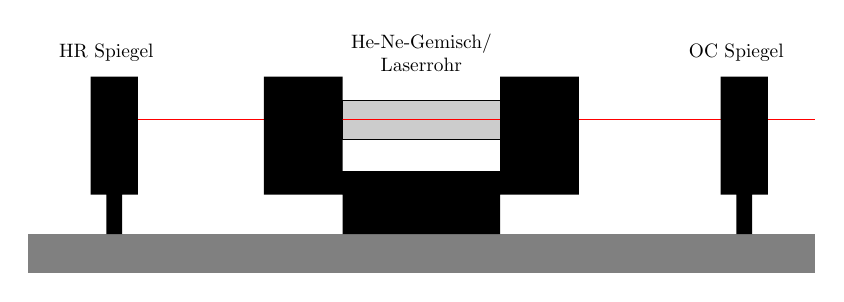
\begin{tikzpicture}
    \fill[white!50!black] (0,0)--(10,0)--(10,0.5)--(0,0.5)--cycle;
    \filldraw[fill=black!20!white] (4,2.2)--(6,2.2)--(6,1.7)--(4,1.7)--cycle;
    \node[scale=0.7,align=center] at (5,2.8) {He-Ne-Gemisch/\\Laserrohr};
    \draw[red] (1,1.95)--(10,1.95);

    \fill (1,0.5)--(1,1)--(0.8,1)--(0.8,2.5)--(1.4,2.5)--(1.4,1)--(1.2,1)--(1.2,0.5)--cycle;
    \node[scale=0.7] at (1,2.8) {HR Spiegel};
    \fill (9,0.5)--(9,1)--(8.8,1)--(8.8,2.5)--(9.4,2.5)--(9.4,1)--(9.2,1)--(9.2,0.5)--cycle;
    \node[scale=0.7] at (9,2.8) {OC Spiegel};

    \fill (4,0.5)--(4,1)--(3,1)--(3,2.5)--(4,2.5)--(4,1.3)--(6,1.3)--(6,2.5)--(7,2.5)--(7,1)--(6,1)--(6,0.5)--cycle;
    \end{tikzpicture}
  \caption{Skizze des Versuchsaufbaus}
  \label{fig:aufbau}
\end{figure}


\subsection{Durchführung}
Zunächst wird der Elektromagnet geeicht. Dazu wird mit einer Hallsonde die Abhängigkeit des Magnetfeldes von der Stromstärke
vermessen.

Mit einem Objektiv und der Linse $L_1$ wird das Licht der Cd-Lampe scharf auf den ersten Spalt $S_1$ abgebildet. Die Linse $L_2$
wird so eingestellt, dass ein paralleles Lichtbündel auf das Prisma fällt. Der Duchmesser des Lichtbündels sollte
dabei nicht größer als der des Prismas sein, da ansonsten Strahlungsverluste auftreten.

Mit der Linse $L_3$ wird ein scharfes Bild auf den nächsten Spalt $S_2$ abgebildet. Dieser wird dazu benutzt, eine bestimmte
Wellenlänge auszusuchen. Es wird zuerst die rote Wellenlänge ausgesucht und dann der Polarisationsfilter so eingestellt,
dass nur der $\sigma$-Anteil des Lichtes hindurchgeht.

Die Linse $L_4$ wird so eingestellt, dass sie ein scharfes Bild auf die Lummer-Gehrcke-Platte abbildet.

Das entstehende Interferenzmuster wird mit der Kamera aufgenommen. Es wird dabei ein Bild mit und ein Bild ohne angeschaltetes
Magnetfeld gemacht.

Anschließend wird der blaue Anteil des Spektrums untersucht, wozu der Spalt $S_2$ neu eingestellt wird. Der Polarisationsfilter
wird so eingestellt, dass zunächst der $\sigma$- und anschließend der $\pi$-Anteil betrachtet werden kann.
Ansonsten wird genauso wie bei der roten Linie vorgegangen.


\section{Ergebnisse}
\begin{table}
    \centering
    \caption{Maximale und minimale Amplitude der Spannungspulse am Oszilloskop in Abhängigkeit des Drucks. (Ohne Folie)}
    \label{tab:dichteprofil}
    \begin{tabular}{ccc}
        \toprule
        $p/\si{\milli\bar}$ &$A_{max}/\si{\volt}$ & $A_{min}/\si{\volt}$\\
        \midrule
        122 &11.0    &6.24\\
        218 &5.32    &2.32\\
        185 &8.88    &2.96\\
        143 &9.04    &4.27\\
        173 &8.72    &3.28\\
        235 &6.32    &2.96\\
        242 &5.28    &3.04\\
        \bottomrule
    \end{tabular}
\end{table}

\begin{table}
    \centering
    \caption{Maximale und minimale Amplitude der Spannungspulse am Oszilloskop in Abhängigkeit des Drucks. (Mit 2µm Goldfolie)}
    \label{tab:dichteprofil_Au}
    \begin{tabular}{ccc}
        \toprule
        $p/\si{\milli\bar}$ &$A_{max}/\si{\volt}$ & $A_{min}/\si{\volt}$\\
        \midrule
        115 &7.52    &2.80\\
        129 &7.28    &3.60\\
        138 &7.44    &3.60\\
        159 &7.04    &3.68\\
        180 &5.28    &2.96\\
        190 &4.08    &2.56\\
        214 &5.28    &3.04\\
        205 &4.00    &2.24\\
        165 &5.84    &2.64\\
        152 &6.88    &3.04\\
        \bottomrule
    \end{tabular}
\end{table}

\begin{table}
    \centering
    \caption{Zählratenmessung in Abhängigkeit des Winkels bei Streuung an einer $2\si{\micro\meter}$ Goldfolie}
    \label{tab:streu_gold}
    \begin{tabular}{ccc}
        \toprule
        $N$ & $\Theta/°$ & $t/\si{\second}$\\
        \midrule
        942     &0.0     &150\\
        816     &-1.0    &150\\
        684     &-2.1    &150\\
        1076    &-3.1    &200\\
        656     &-4.0    &200\\
        492     &-5.1    &250\\
        426     &-6.0    &300\\
        435     &-7.0    &400\\
        333     &-8.1    &450\\
        240     &-9.0    &550\\
        269     &-10.0   &700\\
        998     &1.0     &150\\
        1366    &2.0     &200\\
        1323    &3.0     &200\\
        1817    &4.1     &250\\
        1645    &5.1     &300\\
        1645    &6.1     &350\\
        1448    &7.1     &400\\
        1079    &8.1     &400\\
        746     &9.1     &400\\
        587     &10.1    &400\\
        \bottomrule
    \end{tabular}
\end{table}

\begin{table}
    \centering
    \caption{Zählratenmessung in Abhängigkeit des Winkels bei Streuung an einer $2\si{\micro\meter}$ Bismutfolie}
    \label{tab:streu_bismut}
    \begin{tabular}{ccc}
        \toprule
        $N$ & $\Theta/°$ & $t/\si{\second}$\\
        \midrule
        2301    &-0.1    &150\\
        1064    &-1.1    &150\\
        987     &-2.1    &200\\
        837     &-3.1    &250\\
        522     &-4.1    &300\\
        543     &-5.0    &400\\
        207     &-6.0    &400\\
        \bottomrule
    \end{tabular}
\end{table}

\begin{table}
    \centering
    \caption{Zählratenmessung in Abhängigkeit des Winkels bei Streuung an einer $2\si{\micro\meter}$ Platinfolie}
    \label{tab:streu_platin}
    \begin{tabular}{ccc}
        \toprule
        $N$ & $\Theta/°$ & $t/\si{\second}$\\
        \midrule
        1650    &-0.1    &150\\
        1243    &-1.1    &150\\
        1048    &-2.0    &200\\
        583     &-3.0    &250\\
        779     &-4.0    &350\\
        126     &-5.1    &450\\
        45      &-6.0    &450\\
        \bottomrule
    \end{tabular}
\end{table}


\section{Auswertung}
%Für die Fehlerrechung wird die empirische Standartabweichung
%\begin{equation}
%  \sigma = \sqrt{\frac{1}{n-1} \cdot \sum_{i=1}^n(x_i-\overline{x})^2}
%  \label{eqn:Stdabweichung}
%\end{equation}
%und die Gaußsche Fehlerfortpflanzung
%\begin{equation}
%  u_y = \sqrt{\sum_{i=1}^n\left(\frac{\delta y}{\delta x_i}u_x\right)^2}
%  \label{eqn:gauß}
%\end{equation}
%verwendet.
%\begin{figure}
%  \centering
%  \includegraphics{build/plot.pdf}
%  \caption{Plot}
%  \label{fig:plot}
%\end{figure}
%
\subsection{Dichteabhängigkeit}
Aus den abgelesenen Minima und Maxima in Tabelle \ref{tab:dichteprofil} lassen sich die Mittelwerte bestimmen.
Die Maximal- und Minimalwerte werden im Folgenden als die Fehlerintervallgrenzen gewählt.
Der Energieverlust durch das durchqueren der Folie ist proportional zur Amplitudendifferenz der Spannungspulse bei $p=0$.
Da dieser Wert aufgrund endlicher Pumpleistung nicht erreicht werden kann,
wird ein linearer Fit der Form
\begin{equation}
  A(p) = A_0 + bp
\end{equation}
mit der curve\_Fit-Funktion von scipy \cite{scipy} durch die Messwerte beider Messreihen gelegt.
Dieser ergibt die Parameter
\begin{align}
  A_{0,\text{ohne}} &= (12,1 \pm 1,1)\si{\volt}\\
  b_{\text{ohne}}   &= (-3,40 \pm 0,56)\cdot\SI{e-2}{\volt\per\milli\bar}\\
  A_{0,\text{mit}} &= (8,2 \pm 0,9)\si{\volt}\\
  b_{\text{mit}}   &= (-2,22 \pm 0,56)\cdot\SI{e-2}{\volt\per\milli\bar}
\end{align}
und die Plots in Abbildung \ref{fig:dichteprofil}.
Durch den linearen Zusammenhang zur Energie lässt sich der Energieverlust durch die Folie bestimmen
\begin{align}
  \Delta E &= E_{\alpha}\left(1-\frac{A_{0,\text{mit}}}{A_{0,\text{ohne}}}\right)\\
           &= (1,8 \pm 0,5)\si{\mega\electronvolt}
\end{align}
Damit nun die Bethe-Bloch-Gleichung verwendet werden kann, muss noch die mittlere Geschwindigkeit der $\alpha$-Teilchen ermittelt werden.
Dies wird aus der mittleren Energie und der Energie-Geschwindigkeit-Beziehung hergeleiletet.
\begin{align}
  \overline{E} &= \frac{1}{2} E_{\alpha}\left(1 + \frac{A_{0,\text{mit}}}{A_{0,\text{ohne}}} \right)\\
  \overline{v} &= \sqrt{\frac{2\overline{E}}{m_{\alpha}}}\\
               &= (1,49 \pm 0,04)\cdot\SI{e+7}{\meter\per\second}
\end{align}
Desweiteren werden ein paar materialspezifische Größen benötigt (größtenteils entnommen aus \cite{Gold} oder Allgemeinwissen).
Diese sind die Kernladungszahl von Gold $Z=79$ und des $\alpha$-Teilchens $z=2$, die Dichte von Gold $\rho=19,32\, \si{\gram\per\meter\cubed}$
und die Atommasse von Gold $m_G=196,97\,\text{u}$ und die hierraus folgende Atomdichte
\begin{equation}
  n=\frac{\rho}{m_G}=5,9\cdot\SI{e+28}{\per\meter\cubed}
\end{equation}
, sowie die mittlere Ionisierungsenergie $I=Z\cdot 10\si{\electronvolt}$.
Mit diesen Werten und der Gleichung \eqref{eqn:DeltaX} kann nun die Foliendicke
\begin{equation}
  \Delta x = (3,9 \pm 1,1)\cdot\SI{e-6}{\meter}
\end{equation}

\begin{figure}
  \centering
  \includegraphics{build/dichteprofil.pdf}
  \caption{Durchschnittliche Amplitude der Pulse (Balken gehen von Minimum bis Maximum) gegenüber dem Druck in der Streukammer. Schwarz ist ohne Folie, Blau ist mit Folie}
  \label{fig:dichteprofil}
\end{figure}

\subsection{Streuung}
Für die Streuung ergibt aufgrung des differentiellen Wirkungsquerschnitts aus Gleichung \eqref{eqn:dsdo} die Fit-Funktion
\begin{equation}
  N(\Theta) = \frac{C}{\sin^4\left(\frac{\Theta-\Theta_0}{2}\right)}
\end{equation}
und es ergeben sich mit den Daten aus den Tabellen \ref{tab:streu_gold}, \ref{tab:streu_platin} und \ref{tab:streu_bismut}
die Parameter aus Tabelle \ref{tab:Fitparameter}, sowie die Plots aus den Abbildungen \ref{fig:streu_gold}, \ref{fig:streu_platin} und \ref{fig:streu_bismut}.
Für das Gold wurden hierbei nur die Zählraten unter $4\si{\becquerel}$ in den Fit miteinbezogen.
\begin{table}
  \centering
  \caption{Fitparameter der Zählrate-Winkel-Messung}
  \label{tab:Fitparameter}
  \begin{tabular}{c|ccc}
    \toprule
    \diagdown & Gold & Platin & Bismut\\
    \midrule
    $C$         & (2,14 \pm 0,69)\cdot\SI{e-6}{\becquerel} & (1,9 \pm 1,2)\cdot\SI{e-4}{\becquerel} & (8,89 \pm 2,30)\cdot\SI{e-5}{\becquerel} \\
    $\Theta_0$  & 1,65 \pm 0,11                       & 7,19 \pm 1,23                     & 5,54 \pm 0,39                       \\
    \bottomrule
  \end{tabular}
\end{table}
\begin{figure}
  \centering
  \includegraphics{build/streu_gold.pdf}
  \caption{Zählrate in Abhängigkeit des Winkels bei Streuung an einer $2\si{\micro\meter}$ Goldfolie}
  \label{fig:streu_gold}
\end{figure}

\begin{figure}
  \centering
  \includegraphics{build/streu_platin.pdf}
  \caption{Zählrate in Abhängigkeit des Winkels bei Streuung an einer $2\si{\micro\meter}$ Platinfolie}
  \label{fig:streu_platin}
\end{figure}

\begin{figure}
  \centering
  \includegraphics{build/streu_bismut.pdf}
  \caption{Zählrate in Abhängigkeit des Winkels bei Streuung an einer $2\si{\micro\meter}$ Bismutfolie}
  \label{fig:streu_bismut}
\end{figure}

\subsection{Z-Abhängigkeit}
Wird nun die $Z^2$-Abhängigkeit von Gleichung \eqref{eqn:dsdo} überprüft muss der Fitparameter $C$ aus Tabelle \ref{tab:Fitparameter}
gegen der Ordnungszahl $Z$ aufgetragen und mit einem Fit der Form
\begin{equation}
  C(Z) = aZ^2
\end{equation}
gefittet werden.
Es entsteht der Plot in Abbildung \ref{fig:ordnung} und der Parameter
\begin{equation}
  a = (1,54 \pm 0,78)\cdot\SI{e-8}{\becquerel}.
\end{equation}
\begin{figure}
  \centering
  \includegraphics{build/ordnung.pdf}
  \caption{Fit-Parameter $C$ gegenüber der Ordnungszahl $Z$}
  \label{fig:ordnung}
\end{figure}

\section{Diskussion}
Der Literaturwert\cite{literaturwert} für die Aktivierungsenergie in Strontium dotierten Kalium-Bromid Kristallen liegt bei
\begin{equation}
  W_{lit} = \SI{0.66}{\electronvolt}.
\end{equation}
Bei Betrachtung der bestimmten Aktivierungsenergien (Tabelle \ref{tab:alen})
fällt auf, dass beide Methoden auf ein Ergebnis ähnlicher Größenordnung führen.
Allerdings fällt auf, dass die durch Ausgleichsrechnung des Anstiegs des Relaxationsstromes bestimmten Aktivierungsenergien unter denen durch Integration bestimmten liegen.
Beide Methoden liegen insgesamt um den Literaturwert verteilt, auch wenn keiner der Werte mit seinen Unsicherheitsintervallen auf dem Literaturwert liegt.
\begin{table}[H]
  \centering
  \caption{Aktivierungsenergien aus beiden Messmethoden.}
  \label{tab:alen}
  \begin{tabular}{c|c|c|c}
    Anlaufkurve&&Integration&\\
    \hline
    $W_1$ & $W_2$ & $W_3$ & $W_4$\\
    \hline
    $(0,786\pm 0,052)\si{\electronvolt}$ & $(0,429\pm 0,052)\si{\electronvolt}$ & $(1,074\pm 0,017)\si{\electronvolt}$ & $(1,169\pm 0,065)\si{\electronvolt}$ \\
  \end{tabular}
\end{table}

In der Literatur \cite{literaturwert} ist die Relaxationszeit eines Strontium Dipols durch
\begin{equation}
  \tau_{lit} = 4\cdot10^{-14}\si{\second}
\end{equation}
gegeben.
Die berechneten charakteristischen Relaxationszeiten \ref{eq:relax} weisen sehr starke Abweichungen vom Literaturwert auf.
Dies ist vor allem darauf zurückzuführen,
dass sich auch schon sehr kleine Fehler in den Aktivierungsenergien stark auf die errechnete Relaxationszeit fortpflanzen,
da diese Fehler in die Formel \eqref{eq:tau_0} exponentiell eingehen.

Verfahrensunabhängige Fehlerquellen sind hierbei die Schwankung der Heizraten $H$,
welche unter anderem dadurch bedingt sind,
dass zu Beginn des Heizvorganges das Temperaturgefälle zwischen Probe und Umgebung sehr stark ist,
weshalb die Temperatur ohne zu heizen bereits sehr rapide steigt,
wohingegen ab ca. $\SI{50}{\celsius}$ die maximal zur Verfügung stehende Heizleistung aufgebracht werden muss,
um die Heizrate nicht zu sehr fallen zu lassen.
Zudem ist das verwandte Picoampermeter erschütterungssensitiv.


\newpage
\nocite{*}
\printbibliography

\end{document}
